\documentclass{standalone}
\usepackage{tikz}
\usepackage{xcolor}
\usetikzlibrary{patterns, positioning}
\usetikzlibrary{shapes.misc}
\usepackage[outline]{contour}
\contourlength{1.5pt} 


\begin{document}
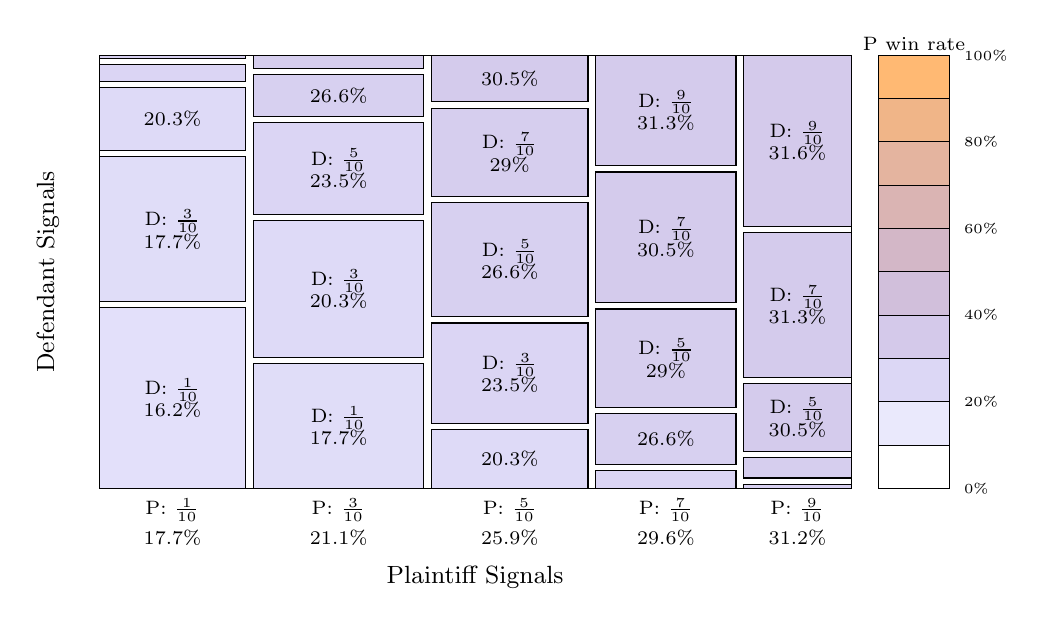
\begin{tikzpicture}
\newcommand{\DFractionOffset}{0.4}
\newcommand{\AxisLabelYAdjust}{-0.235}
\draw[draw=black] (0.6,2) rectangle (10.15,7.5);
\draw[fill=blue!84!orange!16!white!83!white, draw=black] (0.6,2) rectangle (2.4632,4.2917);
\draw (1.531576743200669, 3.14583428124008) node[font=\scriptsize, text=black, align=center] {D: $\frac{1}{10}$\\ 16.2\%};
\draw[fill=blue!82!orange!18!white!82!white, draw=black] (0.6,4.3717) rectangle (2.4632,6.2094);
\draw (1.531576743200669, 5.290538814386773) node[font=\scriptsize, text=black, align=center] {D: $\frac{3}{10}$\\ 17.7\%};
\draw[fill=blue!80!orange!20!white!81!white, draw=black] (0.6,6.2894) rectangle (2.4632,7.0877);
\draw (1.531576743200669, 6.688540874767323) node[font=\scriptsize, text=black, align=center] {20.3\%};
\draw[fill=blue!77!orange!23!white!80!white, draw=black] (0.6,7.1677) rectangle (2.4632,7.3817);
\draw[fill=blue!73!orange!27!white!79!white, draw=black] (0.6,7.4617) rectangle (2.4632,7.5);
\draw (1.531576743200669, 1.6) node[anchor=north, font=\scriptsize, text=black] {17.7\%};
\draw (1.531576743200669, {1.6 + \DFractionOffset}) node[anchor=north, font=\scriptsize, text=black] {P: $\frac{1}{10}$};
\draw[fill=blue!82!orange!18!white!82!white, draw=black] (2.5632,2) rectangle (4.7221,3.586);
\draw (3.64261992772824, 2.7929826476522335) node[font=\scriptsize, text=black, align=center] {D: $\frac{1}{10}$\\ 17.7\%};
\draw[fill=blue!80!orange!20!white!81!white, draw=black] (2.5632,3.666) rectangle (4.7221,5.398);
\draw (3.64261992772824, 4.532007072423244) node[font=\scriptsize, text=black, align=center] {D: $\frac{3}{10}$\\ 20.3\%};
\draw[fill=blue!77!orange!23!white!80!white, draw=black] (2.5632,5.478) rectangle (4.7221,6.6482);
\draw (3.64261992772824, 6.063126210059481) node[font=\scriptsize, text=black, align=center] {D: $\frac{5}{10}$\\ 23.5\%};
\draw[fill=blue!73!orange!27!white!79!white, draw=black] (2.5632,6.7282) rectangle (4.7221,7.2569);
\draw (3.64261992772824, 6.99257187866473) node[font=\scriptsize, text=black, align=center] {26.6\%};
\draw[fill=blue!71!orange!29!white!78!white, draw=black] (2.5632,7.3369) rectangle (4.7221,7.5);
\draw (3.64261992772824, 1.6) node[anchor=north, font=\scriptsize, text=black] {21.1\%};
\draw (3.64261992772824, {1.6 + \DFractionOffset}) node[anchor=north, font=\scriptsize, text=black] {P: $\frac{3}{10}$};
\draw[fill=blue!80!orange!20!white!81!white, draw=black] (4.8221,2) rectangle (6.8084,2.7487);
\draw (5.815267012790379, 2.374374906107276) node[font=\scriptsize, text=black, align=center] {20.3\%};
\draw[fill=blue!77!orange!23!white!80!white, draw=black] (4.8221,2.8287) rectangle (6.8084,4.1006);
\draw (5.815267012790379, 3.464657670711925) node[font=\scriptsize, text=black, align=center] {D: $\frac{3}{10}$\\ 23.5\%};
\draw[fill=blue!73!orange!27!white!79!white, draw=black] (4.8221,4.1806) rectangle (6.8084,5.6258);
\draw (5.815267012790379, 4.903184008091134) node[font=\scriptsize, text=black, align=center] {D: $\frac{5}{10}$\\ 26.6\%};
\draw[fill=blue!71!orange!29!white!78!white, draw=black] (4.8221,5.7058) rectangle (6.8084,6.8284);
\draw (5.815267012790379, 6.267114894741409) node[font=\scriptsize, text=black, align=center] {D: $\frac{7}{10}$\\ 29\%};
\draw[fill=blue!69!orange!31!white!78!white, draw=black] (4.8221,6.9084) rectangle (6.8084,7.5);
\draw (5.815267012790379, 7.204213651254925) node[font=\scriptsize, text=black, align=center] {30.5\%};
\draw (5.815267012790379, 1.6) node[anchor=north, font=\scriptsize, text=black] {25.9\%};
\draw (5.815267012790379, {1.6 + \DFractionOffset}) node[anchor=north, font=\scriptsize, text=black] {P: $\frac{5}{10}$};
\draw[fill=blue!77!orange!23!white!80!white, draw=black] (6.9084,2) rectangle (8.6882,2.2241);
\draw[fill=blue!73!orange!27!white!79!white, draw=black] (6.9084,2.3041) rectangle (8.6882,2.9455);
\draw (7.798311518978024, 2.6247759818687784) node[font=\scriptsize, text=black, align=center] {26.6\%};
\draw[fill=blue!71!orange!29!white!78!white, draw=black] (6.9084,3.0255) rectangle (8.6882,4.2784);
\draw (7.798311518978024, 3.6519560739924275) node[font=\scriptsize, text=black, align=center] {D: $\frac{5}{10}$\\ 29\%};
\draw[fill=blue!69!orange!31!white!78!white, draw=black] (6.9084,4.3584) rectangle (8.6882,6.0185);
\draw (7.798311518978024, 5.188490801078588) node[font=\scriptsize, text=black, align=center] {D: $\frac{7}{10}$\\ 30.5\%};
\draw[fill=blue!69!orange!31!white!78!white, draw=black] (6.9084,6.0985) rectangle (8.6882,7.5);
\draw (7.798311518978024, 6.7992712436616864) node[font=\scriptsize, text=black, align=center] {D: $\frac{9}{10}$\\ 31.3\%};
\draw (7.798311518978024, 1.6) node[anchor=north, font=\scriptsize, text=black] {29.6\%};
\draw (7.798311518978024, {1.6 + \DFractionOffset}) node[anchor=north, font=\scriptsize, text=black] {P: $\frac{7}{10}$};
\draw[fill=blue!73!orange!27!white!79!white, draw=black] (8.7882,2) rectangle (10.15,2.0524);
\draw[fill=blue!71!orange!29!white!78!white, draw=black] (8.7882,2.1324) rectangle (10.15,2.3909);
\draw[fill=blue!69!orange!31!white!78!white, draw=black] (8.7882,2.4709) rectangle (10.15,3.3337);
\draw (9.469087690715217, 2.90231201726414) node[font=\scriptsize, text=black, align=center] {D: $\frac{5}{10}$\\ 30.5\%};
\draw[fill=blue!69!orange!31!white!78!white, draw=black] (8.7882,3.4137) rectangle (10.15,5.2453);
\draw (9.469087690715217, 4.329508214767086) node[font=\scriptsize, text=black, align=center] {D: $\frac{7}{10}$\\ 31.3\%};
\draw[fill=blue!68!orange!32!white!78!white, draw=black] (8.7882,5.3253) rectangle (10.15,7.5);
\draw (9.469087690715217, 6.4126347985856516) node[font=\scriptsize, text=black, align=center] {D: $\frac{9}{10}$\\ 31.6\%};
\draw (9.469087690715217, 1.6) node[anchor=north, font=\scriptsize, text=black] {31.2\%};
\draw (9.469087690715217, {1.6 + \DFractionOffset}) node[anchor=north, font=\scriptsize, text=black] {P: $\frac{9}{10}$};
\node[font=\small, text=black] at (5.375, {1.1 + \AxisLabelYAdjust}) {Plaintiff Signals};
\node[font=\small, text=black, rotate=90] at (-0.050000000000000044, 4.75) {Defendant Signals};
\draw[draw=black] (10.5,2) rectangle (11.4,7.5);
\draw (10.95, 7.65) node[font=\scriptsize, text=black] {P win rate};
\draw[fill=blue!100!orange!0!white!88!white, draw=black] (10.5,2) rectangle (11.4,2.55);
\draw[fill=blue!89!orange!11!white!84!white, draw=black] (10.5,2.55) rectangle (11.4,3.1);
\draw[fill=blue!78!orange!22!white!81!white, draw=black] (10.5,3.1) rectangle (11.4,3.65);
\draw[fill=blue!67!orange!33!white!77!white, draw=black] (10.5,3.65) rectangle (11.4,4.2);
\draw[fill=blue!56!orange!44!white!73!white, draw=black] (10.5,4.2) rectangle (11.4,4.75);
\draw[fill=blue!44!orange!56!white!70!white, draw=black] (10.5,4.75) rectangle (11.4,5.3);
\draw[fill=blue!33!orange!67!white!66!white, draw=black] (10.5,5.3) rectangle (11.4,5.85);
\draw[fill=blue!22!orange!78!white!62!white, draw=black] (10.5,5.85) rectangle (11.4,6.4);
\draw[fill=blue!11!orange!89!white!59!white, draw=black] (10.5,6.4) rectangle (11.4,6.95);
\draw[fill=blue!0!orange!100!white!55!white, draw=black] (10.5,6.95) rectangle (11.4,7.5);
\draw (11.46, 2) node[anchor=west, font=\tiny, text=black] {0\%};
\draw (11.46, 3.1) node[anchor=west, font=\tiny, text=black] {20\%};
\draw (11.46, 4.2) node[anchor=west, font=\tiny, text=black] {40\%};
\draw (11.46, 5.3) node[anchor=west, font=\tiny, text=black] {60\%};
\draw (11.46, 6.4) node[anchor=west, font=\tiny, text=black] {80\%};
\draw (11.46, 7.5) node[anchor=west, font=\tiny, text=black] {100\%};


\end{tikzpicture}
\end{document}